\documentclass[12pt]{book}
\usepackage[width=4.375in, height=7.0in, top=1.0in, papersize={5.5in,8.5in}]{geometry}
\usepackage[pdftex]{graphicx}
\usepackage{amsmath}
\usepackage{amssymb}
\usepackage{tipa}
%\usepackage{txfonts}
\usepackage{textcomp}
%\usepackage{amsthm}
%\usepackage{array}
%\usepackage{xy}
\usepackage{fancyhdr}

\pagestyle{fancy}
\renewcommand{\chaptermark}[1]{\markboth{#1}{}}
\renewcommand{\sectionmark}[1]{\markright{\thesection\ #1}}
\fancyhf{}
\fancyhead[LE,RO]{\bfseries\thepage}
\fancyhead[LO]{\bfseries\rightmark}
\fancyhead[RE]{\bfseries\leftmark}
\renewcommand{\headrulewidth}{0.5pt}
\renewcommand{\footrulewidth}{0pt}
\addtolength{\headheight}{0.5pt}
\setlength{\footskip}{0in}
\renewcommand{\footruleskip}{0pt}
\fancypagestyle{plain}{%
\fancyhead{}
\renewcommand{\headrulewidth}{0pt}
}
%
%\parindent 0in
\parskip 0.05in
%
\begin{document}
\frontmatter
%
\chapter*{\HUGE \center This is not machine learning \\ \Large A relational ethics approach to mathematical modelling}
\thispagestyle{empty}
%{\hspace{0.25in} \includegraphics{./ru_sun.jpg} }
\section*{\large \center Abeba Bihrane and David J. T. Sumpter}
\newpage
\subsection*{\center \normalsize Copyright \copyright 2023 by Abeba Bihrane and David Sumpter}}
\subsection*{\center \normalsize All rights reserved.}
\subsection*{\center \normalsize ISBN \dots}
\subsection*{\center \normalsize \dots Publications}
%
\chapter*{\center \normalsize To }
%
\tableofcontents
%
\mainmatter
%
\chapter{Introduction}
% your text here


\section{This is not...}

While most courses in machine learning and mathematical modelling cover the details of how the methods illustrated above work, our overall purpose is different. {\it This is not a course in machine learning.} It is a rather a course in how to approach the complex reality of the world with machine learning and mathematical modelling tools.

We are going to learn how to position the use of models in a complex world; what we can (and can't) expect to achieve with these models; how to become aware of and describe the limitations of models; and consider situations when it might be better not to use a model at all.  

The title 'this is not' plays, like the artwork that inspires it, on the contradications and ambiguity inherent in modelling. Much of what we will discuss is not the tools of machine learning, but it is the... 


\section{Something}

%


\chapter{Complexity, Modelling and  Relational Ethics}
% your text here
%




This book uses three ideas: (1) critical complexity to assess the limits of models; (2) a modelling approach that combines machine-learning and mechanistic models;  and (3) relational ethics to look at how modellers engage (and sometimes fails to engage) with the world. In this chapter, we give a broad outline of these three ideas, on which we will build upon as we go. 

\section{Critical complexity}

Biological and social systems are complex. The human brain and our other organs; the web of soical interactions over the Internet; the structure of a large buisness or the activities at a University; the ecosystems we live in and are part of; the growth of an embryo; the inner workings of an ant colony or the movement of a fish school. Each one of these systems consist of interacting units that produce patterns far more complex than the units themselves. They are shaped by history. They are messy and difficult to characterise. It is difficult to know where they start and end. 

The scientific challenge is to use the fact that a system is complex to help us better understand it. Sometimes, when we say that a system is complicated when we mean that our insight in to that system is limited. A complex system is difficult to understand. What then can be gained by thinking in terms of complexity science?

The answer to that question, which we underlies the approach taken in this course, comes in the form of {\bf critical complexity}. The term critical complexity arises out of the work of philosophers Paul Cilliers\cite{cilliers2002complexity,cilliers2016critical,cilliers2005complexity}, Alicia Juarrero\cite{juarrero1999dynamicsbook,juarrero2000dynamics} and Rika Preiser\cite{preiser2012problem,preiser2013deconstruction}. These philosophers emphasise the need to embrace the ambiguous, messy, fluid, non-determinable, contextual, and historical nature of complex systems. They describe complex phenomena as unfinalizible and inexhaustible. Complex systems are open-ended, which means there is no way of making an uncontested description of that system. There are always new and different ways of looking at the system.

A way of visualising this description of a complex system is provided by Di Paolo et al. (2018) and reproduced in figure \ref{fig:Complexity}. In the figure, the agents (circles) in a complex system interact (straight arrows) with each other, their environment (wavy lines), which is partially open and ever-changing, and these interactions are continually adjusted (curved arrows) by the agents themselves. 


\begin{figure}[t]
\centering
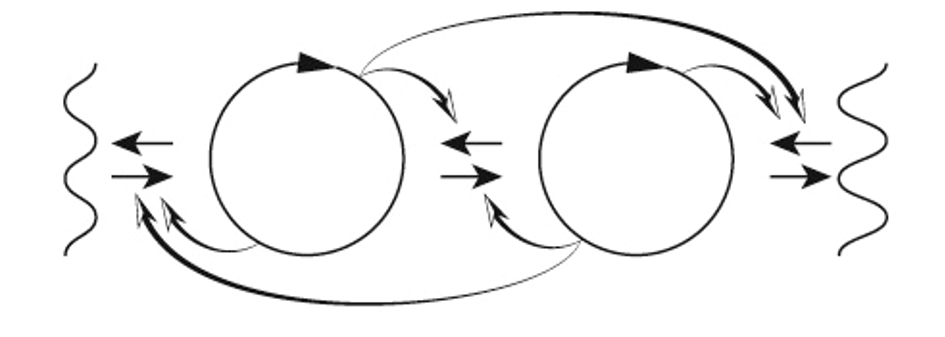
\includegraphics[width=10cm]{Figures/Complexity/Complexity.png}
\centering
\caption{An illustration of a complex system. Adapted from Di Paolo et al. (2018) \cite{di2018linguistic}.  \label{fig:Complexity}}
\end{figure}

If we were to now try to model such a system, or describe some aspect of it, we are forced to make choices about what is inside our model and what is outside. The figure below illustrates such choices, with the blue squares representing ways in which we have closed the system in order to make a model.



\begin{figure}[p]
\centering
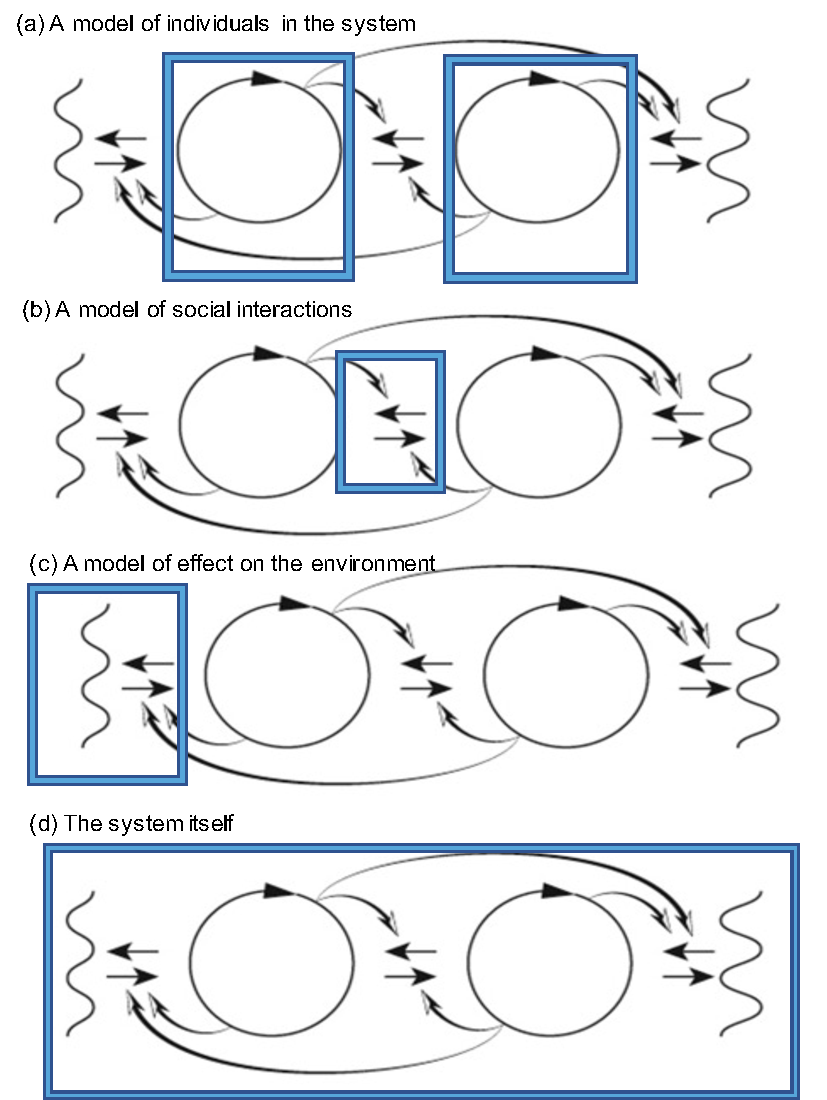
\includegraphics[width=12cm]{Figures/Complexity/ModelsOfComplexity.pdf}
\centering
\caption{Four different ways of modelling a complex system. In terms of (a) individuals (b) social interactions (c) effect of environment or (d) as the entire system. \label{fig:ModelsOfComplexity}} 

\end{figure}


In figure \ref{fig:ModelsOfComplexity} (a) we focus on the individual agents and how they behave, so we create a model which describes their properties and makes simplifying assumptions about how they interact with each other and the world. Here, the agents are inside the model, while their interactions and the environment is outside. In figure \ref{fig:ModelsOfComplexity}(b) we focus instead on the interactions between the agents and in (c) we look at the effect the agents have on their environment. Again, in both these cases, we make simplifying assumptions about things on the outside in order to create a model of the inner workings of one part of the system. 

It is in this way that complex phenomena are unfinalizible and inexhaustible. There are infinitely many ways of building up models of a system, each which leaves something outside. A model is like a snapshot of a landscape and no single snapshot tells the whole story. For modelling the human body, for example, ``a portrait of a person, a store mannequin, and a pig can all be models” \cite{blanchard2011differential}. None is a perfect representation, but each can be the best model for a human, depending on whether one wants to remember an old friend, to buy clothes, or to study anatomy. 

The critical complexity view says that, because complex systems cannot not be completely measured and carry their history with them, there is always a new and different way of looking at them. A few years (or even days) after a portrait is drawn, a person is no longer the same as they were then. We can even talk about their relationship to that portrait, how it shapes their view of the world as they age. The act of modelling, of discussing and analysing changes the world itself. We can never fully capture reality in a single snapshot.

The exception to this rule is illustrated in figure \ref{fig:ModelsOfComplexity}(d), in which we make a model of the entire system. Cilliers argues that such a model {\it is} the system itself. To create such a model, we would need to describe every historical, sociological, biological and physical detail of that system. We would even have to include ourselves studying the system in the model. It is impossible in practice to build such a model and it would be equally impossible to make use of the model or understand what it is telling us.

The use of the word 'critical' in 'critical complexity' thus refers to an activity of criticising a failure to recognise limitations in our models and of thinking carefully about the way we approach modelling. It is this approach we take throughout this book. We see the world as complex in the sense that it is  ambiguous, unfinalizible and inexhaustible. And we are critical of ways in which modellers can fail to recognise complexity and the consequences such failure has on how models are used in society. 

\section{Machine learning and modelling}

\label{sec:mathmodels}

Machine learning is an approach to building models of both simple and complex systems. Let's illustrate how some of these methods work. Not in mathematical detail, but conceptually.


\begin{figure}[t]
\centering
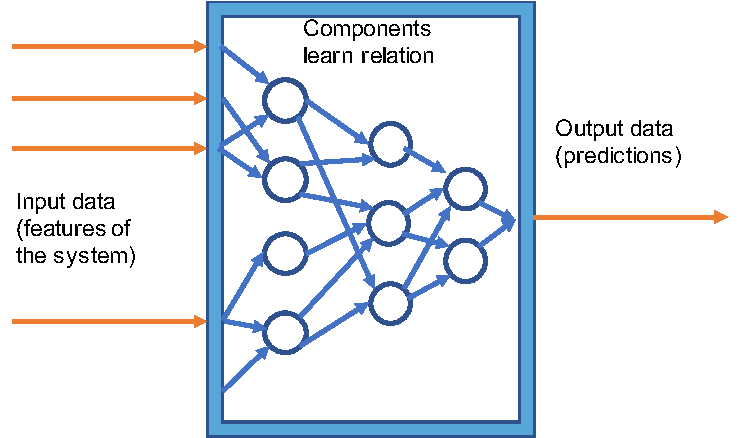
\includegraphics[width=10cm]{Figures/Complexity/SupervisedLearning.pdf}
\centering
\caption{An illustration of the supervised learning problem.   \label{fig:SupervisedLearning}}
\end{figure}


The most well-known method is {\it supervised machine learning}. The idea here is to learn 


In the interactive worksheet (LINK), we give an example of a supervised learning method (logistic regression) in football. MORE  


\begin{figure}[t]
\centering
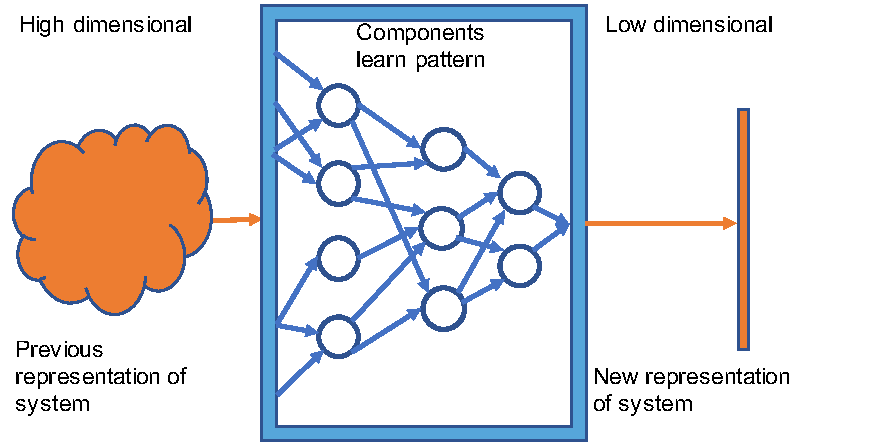
\includegraphics[width=10cm]{Figures/Complexity/UnsupervisedLearning.pdf}
\centering
\caption{An illustration of the supervised learning problem.   \label{fig:UnsupervisedLearning}}
\end{figure}

In {\it unsupervised machine learning} ...

In the interactive worksheet (LINK), we provide an example of categorising a group of people based on their interests using principal component analysis (PCA). MORE HERE.

There are a variety of methods for unsupervised learning. 


In {\it mechanistic modelling}.

\begin{figure}[t]
\centering
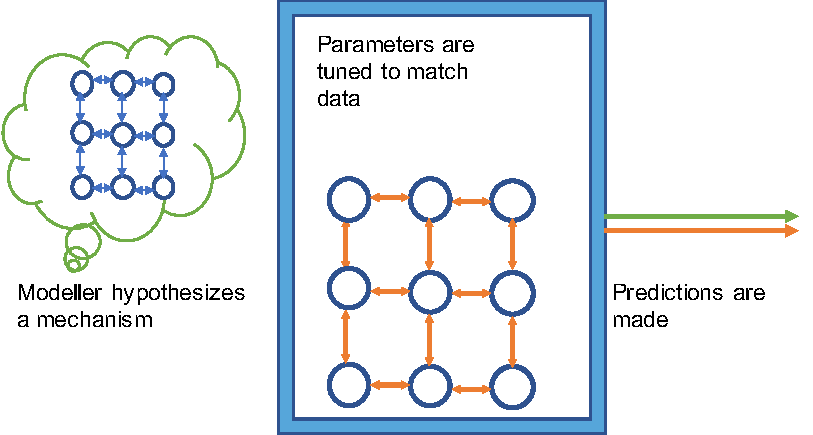
\includegraphics[width=10cm]{Figures/Complexity/Mechanism.pdf}
\centering
\caption{An illustration of a mechanistic model.   \label{fig:Mechanism}}
\end{figure}


In the interactive worksheet (LINK), we provide an example of a mechanistic model of disease spread using an SIR model.

Return to football example. This time with the angle.


OTHER EXAMPLES


\section{An open approach}

In this book, we take an approach to mathematical modelling and machine learning that builds upon figure \ref{fig:ModelsOfComplexity}. We will start from the assumption that there is no unique way of viewing a complex system, but many different views, each of which gives a different insight. Moreover, we assume that applying a mathematical model is akin to using a camera to take a picture of a system. Figures \ref{fig:SupervisedLearning}, \ref{fig:UnsupervisedLearning} and \ref{fig:Mechanism} give an outline of how some these different cameras are built, while the examples in the previous section show in more detail how they work.

In the next chapter we focus on identifying ways in which models close systems. Some systems --- board games, short scale weather prediction, specific datasets and to some extent, biological processes, such as protein folding --- are amenable to closure. We can define where a closed system starts and ends and draw a box around it, which defines its inputs, its outputs and its function. It is conceptually straightforward (although often technically challenging) to build models of these closed systems, which help us understand their properties and predict how they will behave. Then, in chapter \ref{chap:Open}, we look at other systems --- football matches, the Hollywood film industry, the movement of animal groups, outcomes of peoples lives, changes in society--- that are open. It is much harder to build models of these systems, both conceptually and in practice. In many cases it is impossible.

We will argue that the best way to approach complex, open systems is by constructing a wide variety of views. Adopting this approach leads us to a central theme in this book: that when we make choices about which camera to use and which view to take, we cannot escape the fact we are including ourselves in the modelling process. There is no single, objective view to take of these systems. Our values and our ethical choices become part of the modelling process.

Thus, when we look at the technical possibilities and limitations of modelling, we also have to consider ethics and values. We will explain this approach, known as relational ethics, in more detail in chapter \ref{chap:Relational}. But in order to allow the reader to see where we are going with the examples of open and closed systems in the next two chapters, we now give a broad outline of the central idea of relational ethics.

\section{Relational Ethics}

\label{relational}

Relationalism is the idea that morality is an interactive property established between two or more individuals \cite{metz2016relational}. More concretely, the relational approach can be framed in terms of the Ubuntu world view that ``I am
because we are, and since we are, therefore I am'' \cite{mbiti1969african}. Ubuntu is an African philosophy, best known in the West through Archbishop Desmond Tutu’s speech {\it No Future Without Forgiveness}, in which he said, 

\begin{quote}

I am fully me only if you are all you can be. Anger, resentment, nursing grudges corrode, subvert the summum bonum, the great good of the African worldview of communal harmony and they eat away at the very vitals. To forgive is not being altruistic; it is the best form of self-interest. You know what happens to your blood pressure when you are caught in a traffic jam, ``How come they let all those morons drive a car?'' To forgive is good for your physical health as it is for your spiritual health.

\end{quote}

Tutu's description of Ubuntu has parallels to the view of a complex system we saw in figure \ref{fig:Complexity}. It asks us to think of ourselves, when stuck in a traffic jam, as both consisting of a biochemical system (measured by our blood pressure) and as part of an overall social system, our interactions with the other drivers. When analysing the morality of a situation (even one as terrible as Apartheid), Tutu's allegory says we should not just focus on one level, but instead take a view of the various relationships within the system. Just as we should remember that our models capture only one part a larger system or omit detail at a lower level (as in figure \ref{fig:ModelsOfComplexity}), it is a mistake to analyse traffic jams only in terms of ``moron'' drivers. 

Relational frameworks emphasize the importance of dependencies. For example, Kyselo \cite{kyselo2014body} contends that the self is social through and through. We become ourselves and sustain ourselves together with others. Similarly, Bakhtin \cite{bakhtin1984problems} says that only through encounters with others, can we appreciate our own perspectives and form a coherent image of ourselves as a whole entity. By \textit{`looking through the screen of the other’s soul,'} he wrote, \textit{`I vivify my exterior'}. Selfhood and knowledge are evolving and dynamic; the self is never finished – it is an open book \cite{birhane2017descartes}. 

Consider these relational views of our place in society in the context of, for example, predictive policing. The view taken when creating an algorithm to predict crime locations in a city is similar to that of Batman, patrolling a society from the outside and viewing crimes from above in terms of hot spots on a map. Instead of being part of the community, the predictive policing view is disconnected from it. Batman is alienated from those he should serve. As we shall see in chapter \ref{chap:Prediction}, this alienation leads to poor predictions and stereotyping in the use of predictive policing. In order to create successful models of society, we need to consider our own (and our models) place in it. 

In the context of such examples, a particularly important relational approach is Afro-feminism thought. This approach maintains that the most reliable form of knowledge, especially in relation to social and historical injustices, is grounded in lived experience. Patricia Hill Collins \cite{collins2002black}, emphasizes that people do not see the world in abstract forms from a distance, but instead knowledge and understanding emerge from concrete lived experiences. The Afro-feminist approach contends that concrete experiences are primary and abstract reasoning (including modelling) is secondary. Knowing and being are active processes, that are necessarily political and ethical. 

According to the approach outlined by Collins, mathematical models (such as those we discussed in section \ref{sec:mathmodels}) do not take precedence over the actual experience of a person. Modelling cannot be carried out in isolation from others, but should be developed in dialogue with the community it impacts. This is especially important when the type of knowledge in question concerns oppression, structural discrimination, and racism. The Afro-feminist approach maintains that concepts such as ethics and justice need to be grounded in concrete events informed by lived experience of the most marginalized, individuals and communities. We will return to Afro-feminism in more detail in section \ref{sec:Afro-feminism}.

In a similar vein to Afro-feminist thought, the enactive cognitive science theory of participatory sense-making \cite{de2007participatory} advocates for an active and engaged knowing rooted in our relating. A proponent of this position, Hanne De Jaegher \cite{de2019loving}, contends that our most sophisticated human knowing lies in how we engage with each other. In \textit{`Loving and knowing: Reflections for an engaged epistemology'}, De Jaegher \cite{de2019loving} emphasizes that discrete, rational knowing comes at the detriment of \textit{Knowing-in-connection}. Far from a distant and ``objective'' discretising logic, knowing is an activity that happens in the relationship between the knower and the known. Proposing an understanding of human knowing in analogy with loving, De Jaegher argues that in knowing, like loving, what happens is not neutral, general, or universal. Knowers, like lovers, are not abstract subjects but are particular and concrete. ``\textit{Who loves matters}.'' And both loving and knowing take place in the relation between them \cite{de2019loving}. 

Human knowing is based not on purely rational logic, as the rational worldview assumes, but on living and connected know-hows. ``Our most sophisticated knowing'', according to De Jaegher, ``\textit{is full of uncertainty, inconsistencies, and ambiguities}.'' One of the consequences of prioritizing reason is that knowledge of the world and of other people becomes something that is rooted in the individual person’s rational reasoning – in direct contrast to engaged, active, involved, and implicated knowing. Humans are inherently historical, social, cultural, gendered, politicized, and contextualized organisms. Accordingly, their knowing and understanding of the world around them necessarily takes place through their respective lenses.

People are not solo cognizers that manipulate symbols in their heads and perceive their environment in a passive way, as the rationalist view would suggest, but they actively engage with the world around them in a meaningful and unpredictable way. Living bodies, according to Di Paolo, Cuffari, and De Jaegher \cite{di2018linguistic}, are processes, practices, and networks of relations which have ``more in common with hurricanes than with statues''. They are unfinished and always becoming, marked by\textit{``innumerable relational possibilities, potentialities and virtualities''} and not calculable entities whose behaviour can neatly be categorized and predicted in a precise way. Bodies: ``...grow, develop, and die in ongoing attunement to their circumstances... Human bodies are path-dependent, plastic, nonergodic, in short, historical. There is no true averaging of them.'' \citep[p.97]{di2018linguistic}. 

TEXT ABOVE (FROM ABEBA THESIS) SHOULD BE SHORTENED.

Relational perspectives thus view existence in terms of a complex web of social relations. Thus, as in critical complexity, they highlight the impossibility of any unambiguous separation of the real-world, the models we build of a system, and our human values. Afro-feminsism, in particular, emphasises an inherent connection between how one thinks (builds models) and what one does (how models are used and impact society). It is impossible to build a model of reality without taking a specific view and thus adopting an ethical standpoint. Batman beware.


\chapter{Closing a system}
% your text here
%




Use 'closed part of a system'. "We close a system, or we keep an open approach"

The part of the system we have closed can still be complicated. 

In this chapter we use the idea of a closing a system, to help us think about the different systems modelled using machine learning and other mathematical tools. We start by showing that we can close systems do exist in the form of games, experiments in physics and within data sets themselves. Within these closed systems, we can define good practices for modelling them. Indeed, many of the techniques taught on mathematical modelling courses constitute exactly these practices. 

These examples also raise a larger question: what do these closed systems tell us about the real-life, complex, open world? Reality is not a board game or a computer game. A controlled experiment at the atomic or sub-atomic level tells us nothing about our social interactions at work and home. Data about shots in football or the box office success of films is not the same as an actual game of football or a Hollywood movie. The map of an area is not the territory itself.

We will thus broadly separate the systems we model in to approaches two categories: {\it closed systems}, where we have a set of well-defined modelling tools to provide answers about that system, and {\it open systems}, where we have to make a (oftentimes subjective) decision how to close the system in order to apply our tools. The set of closed systems is large, and we will meet many examples during this course, but the set of open systems is even larger and encompasses the biggest challenges 


\section{Board and computer games}

Inside chess there are rules (e.g. white plays first; pawns can move one step or two steps forward on their first move and only one thereafter; the queen can move both backward and forward as well as diagonally and so on). These rules define how we are allowed to act, to play, in every circumstance. As a result, we can write an algorithm which, when shown a chess board with a particular arrangement of pieces, can list all the valid moves. 

In the previous chapter, we stated that the only time we can say we have a complete model of a system is when our model is the the system itself. For chess this is possible. And it is this sense, we say the game of chess is closed. We can capture everything about the game in a model by saying which rules are valid and which are not.

Once we have closed the game in this way, we can also define a mathematical problem within which we calculate, for any given arrangement of pieces on the board, which move will give the best chance of winning the game. It is is thus (in theory) possible to solve chess once and forever and provide the optimal move for any arrangement of pieces. 

In practice, it has also proved possible to build a computer that is better at finding the best moves than humans. The first algorithm that could beat all living humans was Deep Blue. In 1997,

Deep Blue was more closer to a mechanistic model of chess than . 



We can say 

All computer games are closed games. Most, if not all computer games, are played better by a machine learning model than by humans. The exact 



Not all games are completely closed, in the sense that their rules are unambiguous, like those of chess. We will return to this point in chapter \ref{mapterritory} (and also investigate ways in which chess can be made open). For now, we turn our attention to physical, chemical and biological systems. Can some of these be considered as closed?


\section{Physical processes}


Weather models.


\section{Data}

In isolation, a data set constitutes a closed system. This is because data is by its nature an array of 1s and 0s, stored inside a computer (or expressed in a way that would allow it to be stored inside a computer). It is usually possible to create a model of a data set which is simpler than the data itself, in the sense that we can compress the data. For example, when we create a zip file we make the file smaller, but because we can recover the original data again, we know that we have 

Another way of reducing data is to fit a model to it. 


But the data is not the system itself,  




In machine learning, a distinction is made between training and test data. The training data is used to create and fit the model. The test data is then used to measure model performance on unseen data. The reason for taking this approach is to test the degree to which the model is overfit to the specific data on which it was trained. 

We can see the training data as a closed system. When we fit the model to it we are representing that data (and that data only) in the form of a model. When we introduce the test data, we open up the model to a new part of the world on which the model is tested. We test the degree to which the model can deal with that more open part of the world.

While the training/test split reveals the closed nature of the training set, we should remember that the combined training/test set is also closed. Usually, the training and test sets will be randomly sampled from a larger data set. For example, if we have a data set of 1000 shots from football games, 900 might be randomly chosen from these for training and 100 used for testing. Thus, the test/training divide is just an arbitrary division of a closed system in to two parts. 


No matter how much training and testing we have done of a model, we still have to justify how it relates to the open system which constitutes the real world. For example, if we were to apply the expected goals model to a season of football in the same league on which the model is fit, would we consider it a reasonable model? In this case, we probably would.

But would the model still be reasonable ten years from now, 
womens football, youth football, At some point it stops being a reasonable model. 

Model error. 



\cite{waldrop2022beyond}



\section{A case study: Hollywood film data}



The film data set is not the same thing as the Hollywood film industry. 



When we analyse the data set and explain our results to others, we take a specific view. 


- Who created the data set and why?

- Is this just how things are 

Emphasise fact can't capture the entire nature of the system. Depdening on how good and careful cautious you are you are capturing some element.

\section{The two modelling cultures}

\label{sec:twocultures}

In a article published in 2001, Leo Breiman described two cultures in modelling. The first culture assumes that data is generated by a specific {\it mechanism}, while the other concerns itself solely with {\it data}, and treats the mechanism as unknown. We already drew figures illustrating these approaches: figure \ref{fig:Mechanism} illustrates the construction of a mechanistic model, while figure \ref{fig:SupervisedLearning} illustrates a supervised learning approach, where patterns in the data are learnt by the model. The models we created of goals in football --- one based on the geometry of shooting (mechanism), the other based on use of all available data (data-driven) --- illustrate the different approaches. As do the framing of the question ``Can we identifying a Hollywood blockbuster?'' in terms of pure prediction (what the data tells us) or in terms of the role gender has played in Hollywood (mechanism).

Even when we are dealing with closed system, it is not always clear whether a data-driven or mechanistic approach is most appropriate. Breiman's article challenged the statisticians of the time, in asserting that the mechanistic approach ``led to irrelevant theory, questionable conclusions, and has kept statisticians from working on a large range of interesting current problems´´. He showed how random forest models, 

The success of Alpha Zero in creating winning strategies for Go and Chess without any prior information is evidence in favour of the data-driven approach for these and many other game applications. However, some even relatively simple games have remained 


In image analysis, the data-driven approach has proven most successful. 



Attention is all you need...


Any problem 


As Melanie Mitchell writes, “even the most general version, AlphaZero, is not a single system that learned to play Go, chess, and shogi. Each game has its own separate convolutional neural network that must be trained from scratch for its particular game.” 


In conclusion, we note that even within the confines of closed problems there remains debate over whether mechanistic or data-driven approaches are best suited to particular cases. It is though, on balance, it is fair to say that data-driven approaches are now more important for applications involving predictions in closed games and data sets. Many closed problems can be solved without specifying features. For others key features of the problem can be identified, and these (along with some other features that did not appear important in a mechanistic model) can be used to produce highly effective models using neural networks, random forests and other machine learning approaches. 

\section{The map is not the territory}

All mathematical modellers occasionally use language which confuses models for reality. 


\subsection{All models are...}

An often used quote in the context of the relationship between models and reality is George Box aphorism: ``All models are wrong but some are useful''

Box wrote that ``the question you need to ask is not "Is the model true?" (it never is) but "Is the model good enough for this particular application?"'' 

This phrase could be a useful tool for explaining something similar to the map is not the territory idea, but it is not as . To see these, let's look more closely at the use of the words `true´ and `useful'. Imagine you have invited a friend, called Deirdre, for dinner and she have said she will come. You know that Deirdre is usually reliable and often comes to your house. Now imagine that another friend, George, tells you that is isn't true that Deirdre will come, then how you would react? Most of us would be surprised, we would ask George what he knows that we don't. But George doesn't have any extra information, he simply replies that you cannot know for sure that Deirdre will come over, so it isn't true. She might start to feel unwell, remember she has other plans or get hit by a bus on the way to your house, he says. It might be {\it useful} to assume she will come, he says, but it isn't {\it true}!

George is not being particularly helpful here. He is creating a distinction between the words true and useful that are at odds with how we use them. Imagine he did that with every statement you make: `it isn't true   `it isn't true that the sun will come up tomorrow´... 


George Box aphorism isn't particularly true or useful, since it builds on a distinction we seldom make in real life. It encourages a view of modelling that is unhelpfully sceptical, while failing to acknowledge the real challenges. A model should not be judged not primarily in terms of whether it is useful in the sense of `good enough for application', but also in terms of the assumptions it makes, how it relates to previous models, the view it constructs of the world and the consequences for those using it for taking that view.  

The map and territory aphorism allows us to get closer to the essence of what we do when we create a model. Consider, for example, visualisations of population, wealth, on a world map in figure \ref{fig:WealthMap}. The wealth map is distorted from geographic reality, but it captures another form of reality: the inequality in financial wealth across the planet.

\begin{figure}[t]
\centering
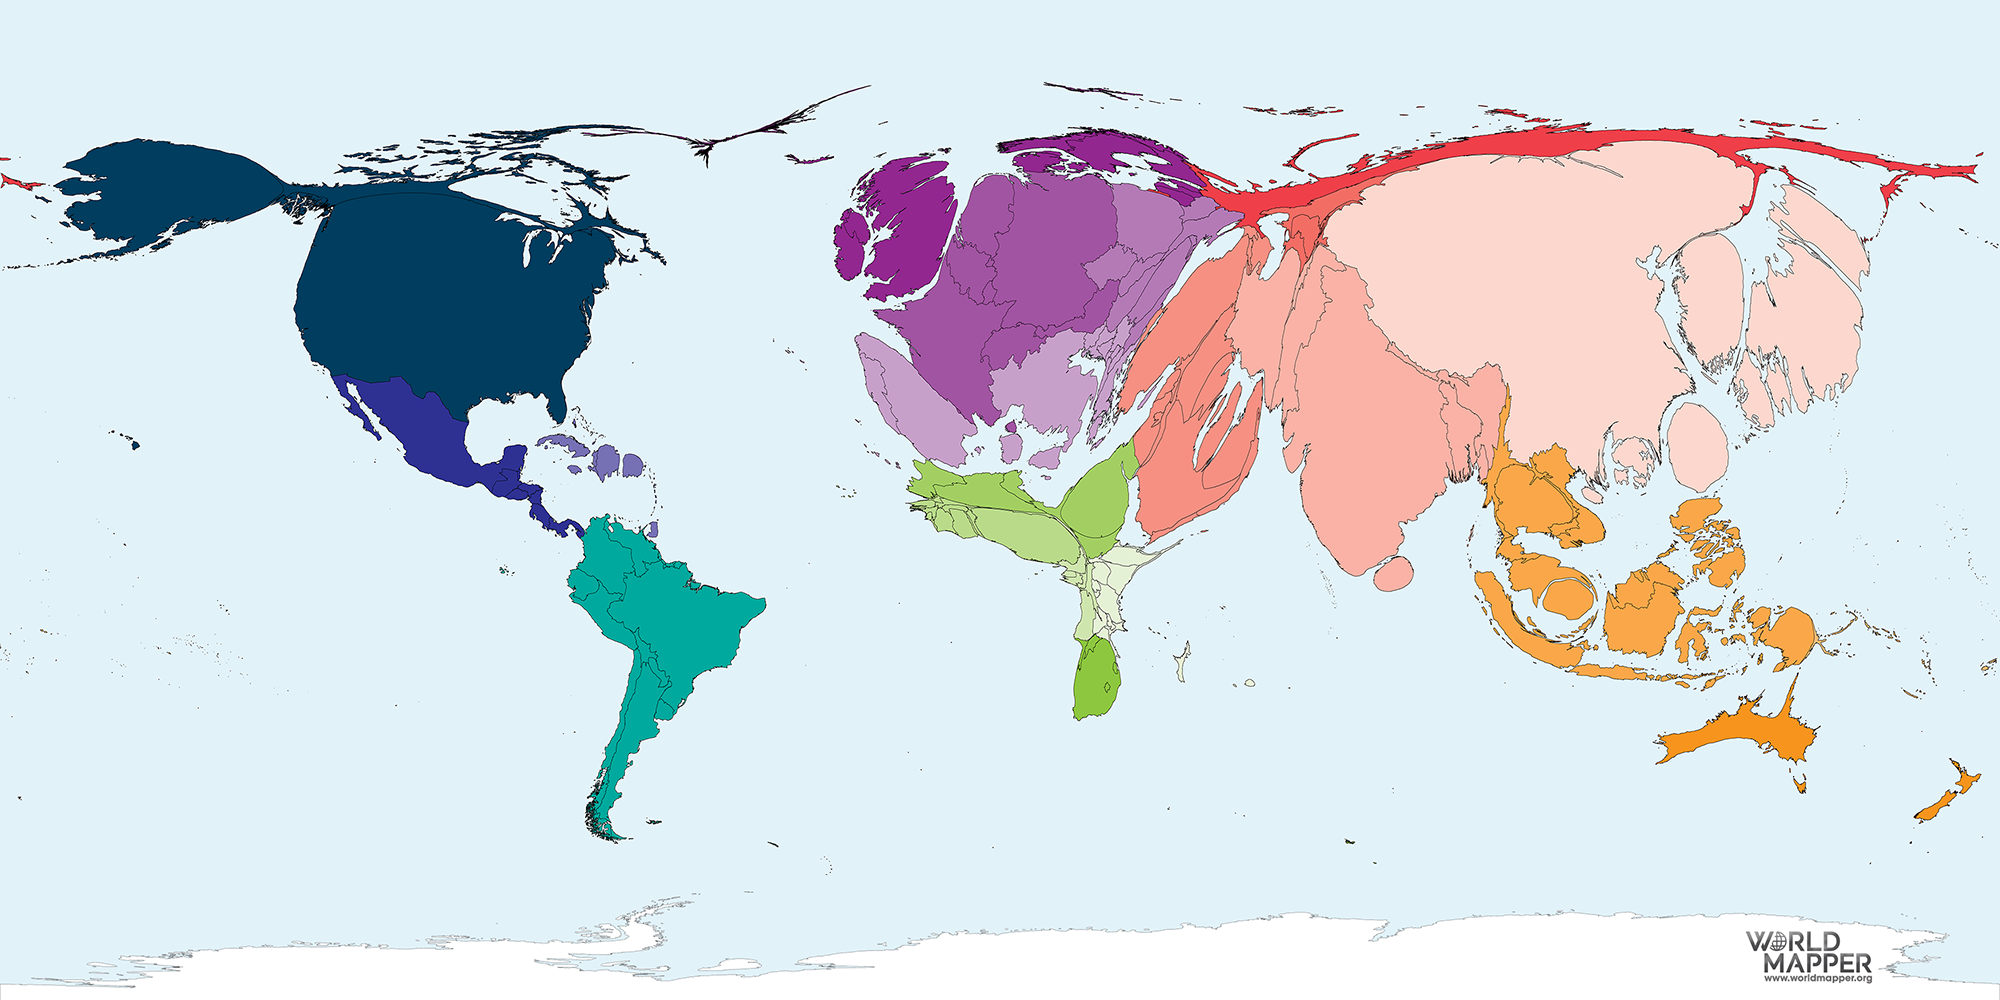
\includegraphics[width=10cm]{Figures/Closed/WealthMap}
\centering
\caption{An illustration of the supervised learning problem.   \label{fig:WealthMap}}
\end{figure}

The question is not whether a model is true or not, but to understand that, like there are many different ways of making maps, there are also many different ways of drawing a map and creating models. Each of them can be a useful (and, in everyday usage of the word, true) guide to the world around us. In the next chapter, we will look at ways of approaching modelling complex, open systems which accounts for this observtaion. 


\subsection{A picture is not enough}

After Deepmind's success with Alpha Zero, one of the research leads on that project David Silver, together with Richard Sutton (a pioneer of reinforcement learning) and other researchers, published an  article claiming that the method they used could be used to explain human abilities, including “knowledge, learning, perception, social intelligence, language, generalisation and imitation”. They even suggested that reinforcement learning could ‘constitute a solution to artificial general intelligence’, the problem of creating a truly human-like machine. Silver acknowledged, in an interview with Wired, that while his hypothesis ‘flies in the face of how a lot of people view AI’, he holds fast to the belief that there is ‘one very clear and simple way to think about all of intelligence … and all of these other things will emerge from that process.’

\begin{figure}[t]
\centering
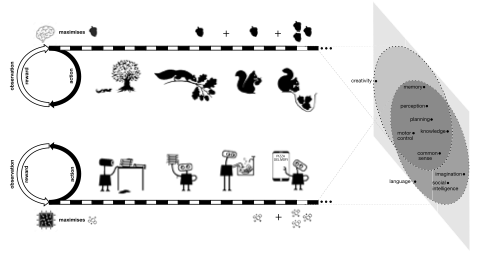
\includegraphics[width=10cm]{Figures/Closed/Squirrel.png}
\centering
\caption{A cartoon representation of a squirrel and a robot, reproduced from Silver et al 2021 \cite{silver2021reward} \label{fig:Squirrel}}
\end{figure}


The argument put forward to support Silver and his colleagues claim uses figure \ref{fig:Squirrel}. They argue that both the robot and the squirrel are examples of reinforcement learning: the squirrel ‘learns’ that getting acorns pays off and evolves more advanced strategies for collecting them and the cleaning robot ‘learns’ that it pays to tidy up and ‘evolves’ to clean its environment.

This cartoon is certainly one valid way of comparing a robot and a squirrel, and biologists sometimes use this paradigm – known as optimal foraging – to understand squirrels’ strategic foraging decisions.  But biologists also know that this paradigm is far from the only way to describe a squirrel. When scientists study animals, they look at: their place in the evolutionary tree; how they evolved to forage on land or at sea; they study physiology and neurology; the viruses and bacteria living inside them; visual and olfactory systems; the chemical processes involved in digesting food; how animal behaviour has been shaped by interactions with humans; and how it is shaped by changing environments and climate change. The ‘squirrel as learning to maximise acorn collection’ is just one of many successful paradigms in biology. 

Figure \ref{fig:Squirrel} creates a visual analogy, mapping a squirrel onto a simulated kitchen robot, by finding one way in which they are similar. Such visual analogies are appealing, but they can also be deceptive, because they deliberately hide complexity. They conceal all the very different ways in which we can look at a squirrel. They hide its complexity. 

Silver and colleagues’ article makes a series of visual analogies. The authors juxtapose five systems: the board game Go (on which reinforcement learning performs well), a robotic agent (in a computational simulation), a physical robot, a squirrel (which they interchange with human behaviour, natural agents, and animals in general) and Artificial General Intelligence (AGI). Their hypothesis is that we can move from Go, to a simulated agent (which they equate to a physical robot), to natural agents, to AGI. As illustrated in figure \ref{fig:ComplexityIncrease}.

\begin{figure}[t]
\centering
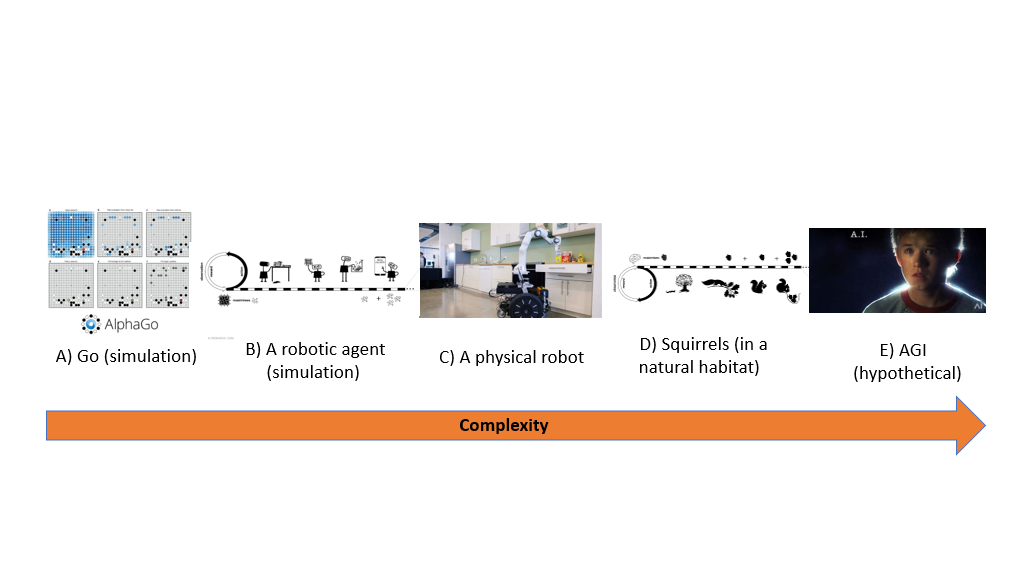
\includegraphics[width=10cm]{Figures/Closed/ComplexityIncrease.png}
\centering
\caption{An illustration of the supervised learning problem.   \label{fig:ComplexityIncrease}}
\end{figure}

Using the approach we have outlined through this chapter we can see the problem of such an argument. Go is a closed game, with well-defined rules and a way of measuring who has won. The cleaning robot simulator is also a closed system. As we discussed in section \ref{sec:twocultures}, it is not currently known whether a problem like this is best solved by 'rewards alone' as proposed by Silver and colleagues (the data-driven approach) or whether a mechanistic model will be needed to build such a robot, even in the closed environment of a computer simulation. 

The important point here, though, is that the jump from a computer simulation to a real-world system means making a move from a closed system to an open system. To claim that a model that works in a computer simulation can be used to tidy living rooms is to confuse the map and the territory.
Current cleaning robots are programmed with additional poop recognition systems, because reinforcement learning can’t teach them that their owners don’t want excrement spread all over the living room floor (spreading dust out before hoovering up is unproblematic, but…). 

Equally, a squirrel is not an Artificial General Intelligence (AGI). There are many different possible models of a human and of a squirrel and there is no way of mapping between the two. We currently lack a clear understanding of what human intelligence is, and the notion of AGI is even more contested and fragmented. There is no clear consensus on how it might be achieved or even if it is possible to build it at all. We will return to this point in chapter \ref{chap:AGI}.




\subsection{Every problem can be opened}




There are ways in which chess can be opened up. For example, consider an older brother playing chess with his little sister. Early in the game, the older sibling might let the younger player retake a move that would have quickly led to her checkmate. They both "break the rules" in order to make a more interesting game. If the younger sister later goes on to place her brother in checkmate, he might remind her that "he let her win." Now, when they report the result to their parents, the outcome is open. The game is no longer just the movement of the pieces itself, but part of a social relation between the players: the older brother still feels he let her win, but he also realises she improved very quickly... Even for him, the game gave rise to an ambiguity. 

%



\chapter{The open approach}
% your text here
%

\label{chap:Open}


Being open to different views of a complex system.


There is no definitive methodology for modelling of complex systems, just a set of plural practices. 

In this chapter we 
focus on several application areas.



\section{Animal behaviour}

The multiple views approach is also adopted when, for example, ant pheromone trails are modelled in terms of cycles of ant activity, formation and topology of the spatial patterns of trail networks, evolution of co-operation and chemical properties of the trails~\cite{sumpter2010collective}. Further examples are found in modelling the growth of tumours, genetic networks and ecological systems. Multiple views are also a prerequisite for modelling (more complex) human social systems~\cite{helbing2010pluralistic}. In adopting an Open ML approach, we simultaneously engage many different frameworks and views of a system, each designed to answer a different sub-question. We take different snapshots of the system and then use each of them to construct a bigger picture of the system. The more snapshots we include, the more complete the bigger picture. ML might help find the sharpest focus of one particular snapshot, but it can not tell us what is a good, overall picture.



\section{Football}

Team sports are more complex compared to board 
games, for example. They involve social, physical, tactical, and mental aspects. Team sports are however less complex than other 
systems such as human societies, 
financial systems, or human brains. 
Modelling the game of football, 
thus allows us to understand some of the challenges involved in modelling open systems, while still dealing with an application of (somewhat) limited scope.

\begin{figure}[t]
\includegraphics[width=11.5cm]{Source/images/Illustration_old.png}
\centering
\caption{Under the Open ML approach, the game of football can be modelled in many different ways. Here we illustrate: the prediction view (top right) simulates the game as a Poisson process; the pitch view uses models to evaluate impact of actions (bottom right); the society view uses the game to understand society at large (bottom left) (figure from \cite{Gregory2021Pace}); and the bio-mechanics view studies physical processes (top left). \label{football}} 

\end{figure}

A widely used model for predicting the outcome of a football match is Poisson regression~\cite{dixon1997modelling}. The central idea is that goals in the match 
are independent, occurring at a rate which depends on the relative quality of the teams and which can be estimated using regression methods.
This model is used by professional gamblers and bookmakers, since it outperforms betting strategies of the customers of the bookmakers (see e.g.~\cite{spann2009sports}). It is possible to include more factors, including events during the match, for example, in a neural network to improve predictions, giving a \textit{prediction} view of the game.

The prediction view is of little use to the players, who will have some sense of the strength of their opponents, and thus whether or not their team is likely to win, but can't be helped by a model (ML or otherwise) which sets probabilities to the outcome. Those playing the game want to understand specific details of their opponents' and their teammates' play which they can exploit during the match. Models that provide these insights can be found, with help of ML, through concepts such as pass probability and pass values, which (using historical data) evaluate the quality of actions~\cite{fernandez2019decomposing,sumpter2016soccermatics}. 

There are many other levels and dimensions to football, as Figure~\ref{football} shows. For example, the \textit{bio-mechanics} view looks at the body kinematics of players~\cite{ibrahim2019kinematic}. One example of the \textit{societal} view is statistical analysis of refereeing to reveal discrimination 
in decisions made~\cite{gallo2013punishing}. Another is the use of computer vision to investigate how sports commentators use words, such as `pace' and `power', when describing players with non-white backgrounds while words such as `hard work', 'effort' and 'mental skill' are used to describe white players. For example,~\cite{Gregory2021Pace} looked at how commentators described events on the pitch when they could and couldn't identify the ethnicity of the players.

Closed and Partially Open ML models can be, and are used in the approach outlined above, in the sense that regression, neural networks, and other methods are used to fit data. But their usage is secondary to finding different views of the sport, taken from different perspectives. Finding a view is sometimes referred to in ML as feature selection. But this terminology places the ML model as primary and the features as secondary. The problem with framing this process as feature selection is that it gives the model itself an aura of neutrality to which subjectively chosen features are added. In fact, the open-ended process of model building is always a necessarily value-laden endeavour. The Open ML approach, which we emphasize, places the ML model as a tool for fitting data, once we have found the view we are interested in. Open ML, then, is about finding a useful view for a certain problem, and combining the views to get an overall understanding of the system. The usefulness of the view subsequently cannot be entirely divorced from the modeller's objectives, motivations, and perspectives.  

\section{Human social behaviour}




\chapter{Relational ethics}
% your text here
%


Over the previous two chapters we have built an approach to modelling which is open to changing its position in order to view systems in multiple ways. This approach encourages taking in to account many different points of view and discourages taking a single, universal perspective. Different useful views of a system are combined to get an overall understanding of the system.

This open-ended process of model building is necessarily value-laden endeavour.  We already saw an indication of this in our example of Hollywood film data: the same data could be used to predict blockbusters or to reflect over discrimination in the film industry. We also saw it when we discussed predictive policing (a subject to which we will return in this chapter). In the coming chapters we will see many more such examples of values. But first, in this chapter, we look in more depth at the relational approach and discuss how it can be used to help incorporate ethical thinking in to an open approach to modelling. 

\section{Afro-feminism} 

\label{sec:Afro-feminism}
\begin{displayquote}
``Knowledge without wisdom is adequate for the powerful, but wisdom is essential for the survival of the subordinate.'' Patricia Hill Collins \cite{collins2002black} \\
\end{displayquote}

We already introduced the relational approach in section \ref{sec:relational}. These include Ubuntu, ... enactive cognitive science and Afro-feminism. It is the latter of these which we look at more closely now, before (in the next section) using it to ground a relational ethics approach which aligns with the open modelling approach we looked at in the previous chapter.

It might, to some readers, appear unusual that we choose Afro-feminism around which to build an ethical approach to machine learning. After all, the writers who developed Black feminist thought were not initially concerned with the best way to use mathematical models. However, these writers were engaged in describing a way of thinking that resisted universalism. Moreover, they were concerned with describing the importance of practice and lived experience in the accumulation of knowledge. And they did so with an intimate knowledge of how inequality and discrimination can be perpetrated by systems when lived experience is neglected. Out of all of the relational approaches it is thus, Afro-feminism thought that offer us most when in providing concrete tools upon which we can build a relational approach. 

Syliva Tamale 


In this section, we detail the above points in more detail, with reference, in particular, to the work by two prominent advocates of Afro-feminist epistemology, Patricia Hill Collins and bell hooks. Then in the next section, we build these in to our own relational ethics approach to machine learning and mathematical modelling.

Drawing on core differences between the dominant Western tradition and the Afro-feminist perspective, Collins broadly identifies two types of knowledge about the world: \textit{book learning} and \textit{wisdom}. For Collins, book learning is reasoning about the world made from a distance in a rational way. This form of knowledge aspires to arrive at ``the objective truth'' that transcends context, time, specific and particular conditions. Wisdom, on the other hand, comes from concrete lived experience. It does not have an ambition to unify, but rather to document our experiences. Wisdom grows as we experience life, but is never complete.


ABEBA: I HAVE MADE CHANGES HERE TO ADDRESS DOUBLE USAGE OF KNOWLEDGE IN YOUR THESIS TEXT. OK?

Collins emphasizes that people are not passive cognizers that contemplate and grasp the world in abstract forms from a distance knowledge. Understanding instead emerges from concrete lived experiences \cite{collins2002black}. Formal education is thus not the only route to knowledge and in many cases is not the most important. Wisdom should be given high credence in assessing knowledge claims.  

For Collins, wisdom takes for granted that there exists an inherent connection between what one does and how one thinks. EXAMPLE. bell hooks \cite{hooks1989talking} (following a pedagogical approach proposed by Paulo Freire \cite{freire1996pedagogy}) emphasises taking a subject to subject approach, in contrast rather than as subject to object approach. When we undertake to study a social system, in particular, we should acknowledge our part of it: we should see ourselves as one subject addressing another subject. By resisting seeing the account of any one subject as ``definitive'' or ``authorative'', we ``create a climate where scholarship from diverse groups ... flourish[es] and [are] better able to appreciate the significance of scholarship that emerges from a particular race, sex, and class perspective.'' (page 45, \cite{hooks1989talking}). Our socio-cultural background --- often refered to as our identity --- necessarily plays a role in how we study another subject.  


The type of wisdom described by Collins is not worked out in isolation from others, but is developed in dialogue with the community. Patricia Hill Collins \cite{collins2002black} gives several examples in the context of African American culture which illustrate this. DISCUSSION page 261 and CHURCH page 263. ....



The distinction between book-learnt knowledge and wisdom experienced through life is especially important when the type of knowledge in question concerns \textit{oppression}, \textit{structural discrimination}, and \textit{racism}. At its heart, the Afro-feminist approach to knowing contends that concrete experiences are primary, and abstract reasoning secondary. It is wisdom, and not ``book learning'', that enables one to identify and resist oppression. It follows that concepts such as ethics and justice need to be grounded in concrete events informed by lived experience of the most marginalized, individuals and communities that pay the highest price when injustice is perpetrated. Knowing and being are active processes that are necessarily political and ethical. 

It is only that experience, which can change an unjust system or design a new approach to societal issues. Audre Lorde famously said that ``Those of us who stand outside the circle of this society's definition of acceptable women; those of us who have been forged in the crucibles of difference -- those of us who are poor, who are lesbians, who are Black, who are older -- know that survival is not an academic skill. It is learning how to take our differences and make them strengths. For the master's tools will never dismantle the master's house.'' \cite{lorde2003master} The experience of those who are oppressed is not merely useful in designing systems which can potentially lead to further oppression. It is primary.

\section{Ethics Built on Relationality}

\label{sec:ethics built on}

Let us summarise where we have come so far in this book. We started by acknowledging that complex systems are open-ended: they carry with them their history and a social context. They are ambiguous, messy, fluid, non-determinable, contextual and never completely understood. There are always new and different ways of looking at a complex system, and thus different ways of creating models. In some cases, most notably games or some physical systems, it is possible to close the system off. But there are many more systems, which remain open and for which we can never find a final all-encompasing view.

We then identified two broad approaches (or cultures) in modelling: one which is data-driven and emphasises prediction; the other which emphasises mechanisms and human understanding. For some closed systems, board games and even weather prediction, the data-driven approach often provides the best way of .

For open systems, both data-driven and mechanistic approaches can be employed, but it is here that the benefits of elucidating a mechanism are greatest. The mechanistic approach allows us to discuss and reason about models, compare our assumptions and reach conclusions in a way that cannot be achieved in a purely data-driven approach. The open approach engages us in an active discussion about the complex systems we want to model. As a result, we need to take our values and ethics in to our modelling approach; in the decisions we make about what to include and leave out of a model. In general, the more open a problem is, the more pressing ethical issues become.

It is here relational thinking comes in. We can think of the mathematical modelling itself as primarily book knowledge, a set of methods for building closed models of particular aspects of a system. On the other hand, the way in which we approach a system as a whole requires lived experience and wisdom: an understanding of the design decisions made when we use models and an understanding of the system we are applying our model to. A relational approach prioritises an open dialogue around modelling choices, over the closed knowledge provided by technical details of models.

bell hooks writes that "dialogue implies talk between two subjects, not the speech of subject and object.” \cite{hooks1989talking}. In terms of modelling, such a dialogue involves discussing and comparing the different ways we view a system, rather than silently applying one or a small number models to that system. A participatory discussion should be opened up about how to approach a problem. 

In the following subsections, we provide some principles which can help structure a relational approach. To make these ideas concrete, we consider the, in the context predictive policing: using algorithms to decide which areas of a city police should patrol. Such algorithms are used in many US cities 



 Here, we use predictive policing in order to illustrate the types of questions that relational ethics should ask. We don't necessarily give answers: although we encourage the reader to think of their own. In later chapters of the book, we will use these principles to challenge 

\begin{itemize}
    \item Paragraph the idea itself.  (Abeba can write long, David shorten)
    \item The literature (Abeba loads and loads)
    \item How to ask a question about predictive policing. (David)
\end{itemize}



\subsection{Subject or Object}
\label{sec:subjectobject}

The quote above from bell hooks makes a key distinction between subject and object. The 


In the predictive policing example, the people living in a city become objects to be monitored and controlled. 



\subsection{Disproportionally impacted}

\label{sec:disproportionally}
The harm, bias, and injustice that emerge from algorithmic systems varies and is dependent on the training and validation dataset, the underlying taken for granted assumptions of the model, and the specific context the system is deployed in, amongst other factors. However, one thing remains constant: individuals and communities that are at the margins of society are disproportionally impacted. Some examples include object detection \cite{wilson2019predictive}; search engine results \cite{noble2018algorithms}; recidivism \cite{angwin2016machine}; gender recognition \cite{buolamwini2018gender}; gender classification \cite{hamidi2018gender,barlassee2020}; and medicine \cite{obermeyer2019dissecting}. Wilson et.al.'s findings in \cite{wilson2019predictive}, for instance, demonstrate that object detection systems designed to predict pedestrians display higher error rates identifying dark skin pedestrians while light-skinned pedestrians are identified with higher precision. The use of such systems situates the recognition of subjectivity with skin tone where whiteness is taken as ideal mode of being. Furthermore, gender classification systems often operate under essentialist assumptions and operationalize gender in a trans-exclusive way resulting in disproportionate harm to trans people \cite{keyes2018misgendering,hamidi2018gender}.  


Given that harm is distributed disproportionately and that the most marginalized hold the epistemic privilege to recognize harm and injustice, relational ethics asks that for any solution that we seek, the starting point be the individuals and groups that are impacted the most. This means we seek to centre the needs and welfare of those that are disproportionally impacted and not solutions that benefit the majority. Most of the time this means not simply creating a fairness metric for an existing system but rather questioning what the system is doing, particularly examining its consequences on minoritized and vulnerable groups. This requires us to zoom out and draw the bigger picture. A shift from asking narrow questions such as \textit{how can we make a certain dataset representative?} to examining larger issues such as \textit{what is the product or tool being used for? Who benefits? Who is harmed? What are the factors that our model has taken into consideration (and what factors are left out as irrelevant). And are the factors we failed to consider or deemed irrelevant indeed so?} 

To some extent, the idea of \textit{centring the disproportionally impacted} shares some commonalities with aspects of \textit{participatory design}, where design is treated as a fundamentally participatory act \cite{slavin2016design} and even aspects human-centered design \cite{irani2010postcolonial} where individuals or groups whom technology is supposed to serve are placed at the centre. However, the idea of \textit{centring the disproportionally impacted} goes further than human-centered or participatory design as broadly construed. While the latter approaches can neglect those at the margins \cite{harrington2020forgotten}, shy away from power asymmetries and structural inequalities that permeate the social world, and ``mirror individualism and capitalism by catering to consumer's purchasing power at the expense of obscuring the hidden labor that is necessary for creating such system'' \cite{Lioyd2020} for the former, acknowledging these deeply ingrained structural hierarchies and hidden labour is a central starting point. In this regard, with a great emphasis on asymmetrical power relations, works such as Costanza-Chock \cite{costanza2018design}'s \textit{Design Justice} and Harrington \cite{harrington2020forgotten}'s \textit{The Forgotten Margins} are examples that provide insights into how centring the disproportionately impacted might be realized through design led by marginalized communities. 

%emphasize the importance of participation. Engaging with complex adaptive systems that surround us, Slavin \cite{slavin2016design} for example, stresses that ``every one of us (designers included) are nothing more than participants in''. 

The central implication of this in the context of a justice centred data practice is that minoritized populations that experience harm disproportionately hold the epistemic authority to recognize injustice and harm given their lived experience. Understandings these concepts and building just technologies therefore, needs to proceed from the experience and testimony of the disproportionately harmed. The starting point towards efforts such as ethical practice in machine learning or theories of ethics, fairness, or discrimination needs to centre the material condition and the concrete consequences an algorithmic tool is likely to bring on the historically marginalized. Having said that, these are efforts with extreme nuances and magnitudes of complexity in reality. For example, questions such as `how might a data worker engage vulnerable communities in ways that surface harms, when it is often the case that algorithmic harms may be secondary effects, invisible to designers and communities alike? What questions might be asked to help anticipate these harms?', `how do we make frictions, often the site of power struggles, visible?' are difficult questions but questions that need to be negotiated and reiterated by communities, data workers and model developers. 




\subsection{Modesty}

The first rule of thumb when dealing with complex systems is the realization and acknowledgement that the phenomena that we are modelling does not have one “right” single solution/answer. Any and all answers will always remain incomplete as complex systems are open and dynamic means that they never come to completion. Completion will simply mark the death of a system. This means that we should always be modest with our claims and models. 


A relational approach shifts toward a more humble and modest understanding complex systems such as people, knowledge and social systems. .... This is also a call for rethinking concepts such as data, ethics, models, matrices of oppression, and structural inequalities as inherently interlinked and processual.   

Such an approach cannot be thought of in terms of universal principles or a set of out-of-the-box tools that can be implemented. 


\subsection{Broaden understanding}

Not every human condition is not a problem to be solved. Complex systems, especially, within the domain of human and social affairs constitute long standing questions that have been contemplated for centuries with no clear answers means that 1) your model is not the first one to deal with these questions so go back and lean on the shoulders of giants and 2) these issues are unlikely to be “solved” once and for all. Thus, in approaching, framing, asking and “answering” questions of complex systems, look back at the historical body of work (outside your narrow and technical field) and build on that.       



\subsection{Critical reflection}

The search for irony is an internal process of challenging yourself as a researcher. One example is avoiding the temptation of low hanging fruit: if it feels that a theoretical result, which has no obvious application but is publishable and might attract interest from your peers, is within reach then make a brief note of how it might be solved (either for yourself or published in a blog) and then focus your attentions elsewhere. 
Use a variety of methods: Instead of polishing our own favourite lens and describing how it reflects white light, we should make use of every lens in our camera bag to get a multitude of different pictures and angles on our subject. We should treat the economy or social systems just as we treat the human body in Blanchard et al.’s example: as a portrait, as a mannequin, or as a pig. There are so many different ways to see ourselves and our society, we need to use them all to get as full a picture as possible. Examples can be seen in the study of collective animal behaviour, where different modelling and experimental approaches interact in the study of animal groups (Sumpter, 2010). 




\subsection{Reject notions of neutrality}

Systems cannot be modelled from the view from nowhere. The observer (and her objectives, values, and interests) is necessarily part of the model. When modelling human behaviour and social systems, which are contested and value-laden, there is no neutral lens. The more diverse the perspective, the fuller the picture the model produces.   


\subsection{Create ambitious theory}

????? Qualify for radicallity?

Develop entirely new lenses – radically theories of how to view complex systems. Some pointers in the direction include research in artificial life, using and developing online games where humans interact with simulations and investigating novel cellular automata (see figure 2). The common theme is an open-ended attempt to identify emergent phenomena, without ever trying to close the system with an exhaustive mathematical analysis. Instead of stifling the use of mathematics, a true complexity science pushes us to be more creative, to take risks and allow ourselves to be spectacularly wrong.  


\subsection{Embrace ambiguity}

Complexity science’s gradual slip back into reductive science is driven in part by the desire for control, certainty, universality, and absolute objectivity (again, the view from nowhere) (Birhane, 2021). However, when dealing with the messy, ambiguous and value-laden nature of complex systems, these desires are an illusion. In an academic ecology that rewards a false sense certainty, it is difficult to sell incomplete answers. Acknowledging that we never have a full grasp of complex phenomena or complete description of a system in its entirety — embracing ambiguity, being humble about our models, and being comfortable with “we don’t know” — can create a better culture for everyone.  



\subsection{Acknowledge power dynamics}

Since knowing is a relational affair, who enters into the knower-known relations matters. Within the fields of computing and data sciences, the \textit{knower} is heavily dominated by privileged groups of mainly elite, Western, cis-gendered, and able-bodied white men \cite{broussard2018artificial}. Given that knower and known are closely tied, this means that most of the knowledge that such fields produce is reduced to the perspective, interest, and concerns of such dominant group. Subsequently, not only are the most privileged among us restricted to producing partial knowledge that fits a limited worldview (while such knowledge, tools, models, and technologies they produce are forced onto all groups, often disproportionately onto marginalized people), they are also poorly equipped to recognize injustice and oppression \cite{Berenstain2016}. D'Ignazio and F. Klein \cite{d2020data} call this phenomenon \textit{the privilege hazard}. This means that minoritized populations 1) experience harm disproportionally and 2) are better suited to recognize harm due to their epistemic privilege \cite{on1993marginality} while the reverse holds for those building and deploying models.  

%In approaching knowing as a relational and active practice, we understand it as active, contextual, and placing human relations as central to knowledge and 

\subsection{The Master's tools}


\subsection{Checklists can be reductive}

Very nature of these systems, the list is inexausable. These systems are changing and moving. The number of items you can list is endless. 


\section{Relational versus Rational}

Rational presented as a given. 


Current data practices, for the most part, follow the rational model of thinking where data are assumed to represent the world ``out there'' in a ``neutral'' way. Yet, not only is it fallacious to assume complex social reality can be fully represented by data, the process of data collection, analysis and interpretation of results is a value-laden endeavour. In the process of data collection, for example, the data scientist decides what is worth measuring (making some things visible and others invisible by default) and how. In the process of data cleaning, rich information that provides context about which data are collected and how datasets are structured is stripped away. Emphasizing the importance of contexts for datasets, Loukissas \cite{loukissas2019all} has proposed a shift into thinking in terms of \textit{data settings} instead of \textit{datasets}. 

The rational worldview that aspires to an ``objective'' knowledge from a ``God’s eye view'' has resulted in the treatment of the researcher as invisible, their interests, values, and background as inconsequential. In contrast, for Afro-feminist thought, the researcher is an important participant in the knowledge production process \cite{nnaemeka2004nego}. For Sarojini Nadar \cite{nadar2014stories}, coming to know is an active and participatory endeavour with the power to transform. Consequently, data and our models portray and represent certain mode of reality while leaving out others.   
%narrative research, since it puts story telling at the centre, invites us to consider stories as `data with soul' \cite{nadar2014stories}. 


The relational approach can be contrasted to many Western approaches, which were concerned with finding ways of seperating these three aspects. For example, Descarte ....

Similarly, in the 1920's logical positivism sought to categorise statements we make about the world as being synthetic (about the complex real world), analytical (about the properties of models) and nonsense (about value judgements). 

\subsection{No boundaries}


Before we delve into that, it is worth reemphasising that while the rational worldview tends to see knowledge, people, and reality in general as stable, for relational perspectives, we are fluid, active, and continually becoming. Nonetheless, the relational vs rational divide is not something that can be clearly demarcated but overlaps with fuzzy boundaries. Some approaches might prove difficult to fit in either category while others serve to bridge the gap -- Harding's \cite{harding1992rethinking} \textit{Strong Objectivity} is one such example that links relational and rational approaches. Furthermore, the relational and rational traditions exist in tension with a continual push and pull. For example, complexity science is a school of thought that emerged from this tension.   


\subsection{Language games}

Western philosophy has investigated similar ideas to those contained within Ubuntu. In Anglo-American philosophy, these start with the later work of Ludvig Wittgenstein. He formaulated the idea of langauge games, which very much parallels the approach we take above of taking snapshots of a system.

Postmodernismis sometimes used in terms of derision by some scientists, who portray it as the opposite of a scientific approach. For example,

These criticisms of 
As Cilliers pointed out, in his book Complexity and Postmodernism, 




\chapter{Limits of prediction}
% your text here
%
\ref{chap:Prediction}



\section{Predicting societal outcomes}

Stock market models.

Election results.



\section{Predicting personalities}




\section{Life trajectories}




\section{AI pseudoscience}





\section{Understanding over prediction}
\label{prioritizing understaning}
\begin{displayquote}
``I have never been impressed with claims that structural linguistics, computer engineering or some other advanced form of thought is going to enable us to understand men without knowing them.'' Clifford Geertz \cite{geertz1973interpretation}
\end{displayquote}

%The rationalist tradition, with its tendency for timeless, free-standing, and generalizable knowledge, aspires to establish fundamental laws and timeless theories. Observed commonalities, recurring similarities, and repeated patterns among particular events or behaviours are abstracted to make generalizations and furthermore to forecast the future based on the past. Abstraction, generalization, and universal principles — since the focus is uncovering what remains constant regardless of context, culture, and time — means specific, concrete, particular, and contextual understanding grounded in active and reciprocal relations are devalued. According to Geertz the desire to formulate general theories on the one hand and the need to gain deep understanding of particular and contextual events and behaviors constitute an irremovable tension within the human sciences. The further theory goes, the deeper the tension. Geertz contests that theories and generalizations inevitably lack deep and contextual understanding of human thought. Theoretical disquisitions stand far from the immediacies of social life. And any generalization or theory construction in the absence of deep understanding grounded in the concrete and particular, is vacuous.

The rationalist tradition's tendency toward timeless and generalizable knowledge aspires to establish timeless laws and generalizable theories. This pipeline takes observed commonalities, recurring similarities, and repeated patterns among past events or particular behaviours and abstracts them into generalizations that can be applied toward forecasting the future. Because the rationalist's focus is to uncover what remains constant regardless of context, culture, and time, the rationalist view embraces abstraction, generalization, and universal principles at the expense of concrete, particular, and contextual understanding — that is, knowledge grounded in active, concrete, and reciprocal relationships. According to Geertz \cite{geertz1973interpretation}, the desire to formulate general theories is in an \textit{irremovable tension} with the need to gain deep understanding of particular and contextual events and behaviors. The further theory goes, the deeper the tension. Theories and generalizations inevitably lack deep and contextual understanding of human thought. Theoretical disquisitions stand far from the immediacies of social life. Any generalization or theory constructed in the absence of deep understanding, not grounded in the concrete and particular, is vacuous.

On a similar note, the Russian philosopher Mikhail Bakhtin refers to the manner in which abstract general rules are derived from concrete human actions and behaviours as \textit{theoretism}. Bakhtin argues such attempts to abstract general rules from particulars ``loses the most essential thing about human activity, the very thing in which the soul of morality is to be found'' which Bakhtin calls, the \textit{``eventness''} of the event \cite{morson1989rethinking}. \textit{Eventness} is always a particular, and never exhaustively describable in terms of rules. In order to understand people, we must take into account \textit{``unrepeatable contextual meaning''}. Likewise, the historian of science Lorraine Daston contends that the strive for a universal law is a predicament that does not stand against unanticipated particulars since no universal ever fits the particulars \cite{daston2018calculation}. Commenting on current machine learning practices Daston \cite{Gross2020} explains: ``machine learning presents an extreme case of a very human predicament, which is that the only way we can generalize is on the basis of past experience. And yet we know from history —-- and I know from my lifetime —-- that our deepest intuitions about all sorts of things, and in particular justice and injustice, can change dramatically.''

While the rationalist tradition tends to aspire to produce generalizable knowledge disentangled from historical baggage, context, and human relations, relationalist perspectives strive for concrete, contextual, and relational understanding of knowledge, human affairs, and reality in general. Data science and machine learning systems sit firmly within the rationalist tradition. The core of what machine learning systems do can be exemplified as clustering similarities and differences, abstracting commonalities, and detecting patterns. Machine learning systems ``work'' by identifying patterns in vast amounts of data. Given immense, messy, and complex data, a machine learning system can sort, classify, and cluster similarities based on seemingly shared features. Feed a neural network labelled images of faces and it will learn to discern faces from not-faces. Not only do machine learning systems detect patterns and cluster similarities, they also make predictions based on the observed patterns \cite{o2013doing}. Machine learning, at its core, is a tool that predicts. It reveals statistical correlations with no understanding of causal mechanisms. 

Relational ethics, in this regard, entails moving away from building predictive tools (with no underlying understanding) to valuing and prioritizing in-depth and contextual understanding of the phenomena that we are building predictive models for. This means we examine the patterns we find and ask why we are finding such patterns. This in turn calls for interrogating contextual and historical norms and structures that might give rise to such patterns instead of using the findings as input towards building predictive systems and repeating existing structural inequalities and historical oppression. 

If we go back to the Bayesian models of inference mentioned in Section \ref{rationality}, we find that such models are prone to amplification of socially held stereotypes. Repeating Horgan \cite{Bayes2016}'s point: ``Embedded in Bayes’ theorem is a moral message: If you aren’t scrupulous in seeking alternative explanations for your evidence, the evidence will just confirm what you already believe.'' A data practice that prioritizes understanding over prediction is one that interrogates prior beliefs instead of using the evidence to confirm such belief and one that seeks alternative explanations by placing the evidence in a social, historical, and cultural context. In doing so, we ask challenging but important questions such as `to what extent do our initial beliefs originate in stereotypically held intuitions about groups or cultures?', `why are we finding the ``evidence'' (patterns) that we are finding?', and `how can we leverage data practices in order to gain an in depth understanding of certain problems as situated in structural inequalities and oppression?' 


%This in practice might look like, for example, investigating (with the aim to understand) 

%This section could do with a bit of "cleaning up", I think, in terms of what each § aims to and actually does. E.g. the penultimate § seems to begin to talk about relational approaches, but then ends on typical ML and data science approaches again. 
%Also, I wonder if what you say in the final § here can be extended. What is it that data science can do in a relational approach? (Or maybe that comes in the next section... I'll read on.)


\section{Impossibility of automating ambiguity}


AI and ML systems that cluster, sort, and predict human behaviour and action, are force order, equilibrium, and stability to the active, fluid, messy, and unpredictable nature of human behaviour and the social world at large. 

We are always already situated within social practices, and the way we interact with and make sense of the world needs to be understood against this background.

 We are fully embedded and enmeshed with our designed surroundings and we critically depend on this embeddedness to sustain ourselves. Furthermore, our historical paths, the moral and political values that we are embedded in, constitute crucial components that contribute to who we are. People, as complex adaptive systems, are \textit{non-totalisable}. The idea of defining the person once and for all, drawing simple classifications, and making accurate predictions thus appears a futile endeavour. In complexity science terms, human beings and their behaviour are complex adaptive phenomena whose precise pathway is simply unpredictable~\citep{juarrero2000dynamics}.

 




\chapter{Fairness}
% your text here
%






\section{Fairness Through Awareness}

Imagine your colleagues have created a supervised machine learning model to find people who might be interested in studying at a university in Sweden, based on their activity on a social networking site. Their algorithm either recommends or doesn't recommend the course to users. They have tested it on two different groups of people (600 non-Swedes and 1 200 Swedes), all of whom would be eligible for the course and have given permission for their data to be used. As a test, your colleagues first applied the method, then asked the potential students whether or not they would be interested in the course. To illustrate their results, they produced the confusion matrices shown in Table \ref{tab:SwNonSw} for non-Swedes and Swedes.


\begin{table}
\caption{Proportion of people shown and/or interested in a course for an imagined machine learning algorithm. The top table is for non-Swedes (in this case we can think of them as citizens of another country, but who are eligible to study in Sweden); the bottom table is for Swedes. \label{tab:SwNonSw}}\index{confusion matrix}
	\centering
\smallskip
		\begin{tabular*}{\textwidth}{@{\extracolsep{\fill}}r|cc@{\extracolsep{\fill}}}
\hline
			&  Not Interested &  Interested  \\
			\textbf{Non-Swedes} &  ($y=-1$)&  ($y=1$) \\
\hline
			Not recommended course ($\yhat(\bx) = -1$)  & TN = $300$ & FN = $100$ \\
			Recommended course ($\yhat(\bx) = 1$) & FP = $100$ & TP = $100$  \\
\\
			&  Not Interested &  Interested  \\ %\hline
\textbf{Swedes}  &   ($y=-1$)&  ($y=1$) \\ \hline
			Not recommended course ($\yhat(\bx) = -1$)  & TN = $400$ & FN = $50$ \\
			Recommended course ($\yhat(\bx) = 1$)& FP = $350$ & TP = $400$  \\
\hline
		\end{tabular*}
		%\label{tab:loss
		\vspace{-2em}
\end{table}	
	
	
Let's focus on the question of whether the algorithm performs equally well on both groups, non-Swedes and Swedes. We might call this property `fairness'. Does the method treat the two groups fairly? To answer this question, we first need to quantify fairness. One suggestion here would be ask if the method performs equally well for both groups. Referring to \cref{tab:confmatterm}, and \cref{ch:evaluation} in general, we see that one way of measuring performance is to use misclassification error. For \cref{tab:SwNonSw}, the misclassification error is $(100+100)/600=1/3$ for non-Swedes and $(50+350)/1\,200=1/3$ for Swedes. It has the same performance for both categories.

\enlargethispage{-\baselineskip}

It is now that alarm bells should start to ring about equating fairness with performance. If we look at the false negatives (FN) for both cases, we see that there are twice as many non-Swede FN cases as Swedish cases (100 vs. 50), despite their being twice as many Swedes as non-Swedes. This can be made more precise by calculating the false negative rate (or miss rate), i.e. FN/(TP+FN) (again see \cref{tab:confmatterm}). This is $100/(100+100)=1/2$ for non-Swedes and $50/(400+50)=1/9$ for Swedes. This new result can be put in context by noting that Swedes have a slightly greater tendency to be interested in the course (450 out of 1 200 vs. 200 out of 600). However, an interested non-Swede is 4.5 times more likely \textit{not} to be recommended the course than an interested Swede. A much larger difference than that observed in the original data.

%\enlargethispage{1em}

There are other fairness calculations we can do. Imagine we are concerned with intrusive advertising, where people are shown adverts that are uninteresting for them. The probability of experiencing a recommendation that is uninteresting is the false positive rate, FP/(TN+FP). This is $100/(300+100)=1/4$ for non-Swedes and $350/(350+400)=7/15$ for Swedes. Swedes receive almost twice as many unwanted recommendations as non-Swedes. Now it is the Swedes who are discriminated against!

This is a fictitious example, but it serves to illustrate the first point we now want to make: \textit{There is no single function for measuring fairness}. In some applications, fairness is perceived as misclassification; in others it is false negative rates, and in others it is expressed in terms of false positives. It depends strongly on the application. If the data above had been for a criminal sentencing application, where `positives' are sentenced to longer jail terms, then problems with the false positive rate would have serious consequences for those sentenced on the basis of it. If it was for a medical test, where those individuals not picked up by the test had a high probability of dying, then the false negative rate is most important for judging fairness.

As a machine learning engineer, you should never tell a client that your algorithm is fair. You should instead explain how your model performs in various aspects related to their conception of fairness. This insight is well captured by Dwork and colleagues' article, `Fairness Through Awareness' \parencite{dwork2012fairness}, which is recommended further reading. Being fair is about being aware of the decisions we make both in the design and in reporting the outcome of our model.


\section{Complete Fairness Is Mathematically Impossible} \label{sec:nofairness}

We now come to an even more subtle point: \textit{It is mathematically impossible to create models that fulfil all desirable fairness criteria}. Let's demonstrate this point with another example, this time using a real application. The Compas algorithm was developed by a private company, Northpointe, to help with criminal sentencing decisions. The model used logistic regression with input variables including age at first arrest, years of education, and questionnaire answers about family background, drug use, and other factors to predict an output variable as to whether the person would reoffend \parencite{sumpter2018outnumbered}. Race was not included in the model. Nonetheless, when tested -- as part of a a study by Julia Angwin and colleagues at Pro-Publica \parencite{larson2016we} -- on an independently collected data set, the model gave different predictions for black defendants than for white. The results are shown in the form of a confusion matrix in Table \ref{ch12:tab12.2}, for re-offending over the next two years.

\begin{table}[!t]
\caption{Confusion matrix for the Pro-Publica study of the Compas algorithm. For details see \textcite{larson2016we}.}\label{ch12:tab12.2}
\smallskip		
\centering
		\begin{tabular*}{\textwidth}{@{\extracolsep{\fill}}r|cc@{\extracolsep{\fill}}}
\hline
			\textbf{Black defendants} &  Didn't reoffend ($y=-1$)&  Reoffended ($y=1$) \\ \hline
			Lower risk ($\yhat(\bx) = -1$)  & TN = $990$ & FN = $532$ \\
			Higher risk ($\yhat(\bx) = 1$)  & FP = $805$ & TP = $1\,369$  \\
\\
			\textbf{White defendants} &  Didn't reoffend ($y=-1$)&  Reoffended ($y=1$) \\ \hline
			Lower risk ($\yhat(\bx) = -1$)  & TN = $1\,139$ & FN = $461$ \\
			Higher risk ($\yhat(\bx) = 1$)  & FP = $349$ & TP = $505$  \\
\hline
		\end{tabular*}
		%\label{tab:loss}
\end{table}		
	
Angwin and her colleagues pointed out that the false positive rate for black defendants, $805/(990+805)=44.8$\%, is almost double that of white defendants, $349/(349+1\,139)=23.4$\%. This difference cannot be accounted for simply by overall reoffending rates: although this is higher for black defendants (at 51.4\% arrested for another offence within two years), when compared to white defendants (39.2\%), these differences are smaller than the differences in false positive rates. On this basis, the model is clearly unfair. The model is also unfair in terms of true positive rate (recall). For black defendants, this is $1\,369/(532+1369)=72.0$\% versus $505/(505+461)=52.2$\% for white defendants. White offenders who go on to commit crimes are more likely to be classified as lower risk.

\enlargethispage{2em}

In response to criticism about the fairness of their method, the company Northpointe countered that in terms of performance, the precision (positive predictive value) was roughly equal for both groups: $1\,369/(805+1369)=63.0$\% for black defendants and $505/(505+349)=59.1$\% for white \parencite{sumpter2018outnumbered}. In this sense the model is fair, in that it has the same performance for both groups. Moreover, Northpointe argued that it is precision which is required, by law, to be equal for different categories. Again this is the problem we highlighted above, but now with serious repercussions for the people this algorithm is applied to: black people who won't later reoffend are more likely to classified as high risk than white people.

Would it be possible (in theory) to create a model that was fair in terms of both false positives and precision? To answer this question, consider the confusion matrix in Table \ref{ch12:tab12.3}.
	\begin{table}[!t]
\caption{Generic confusion matrix.}\label{ch12:tab12.3}
\smallskip
\centering
		\begin{tabular*}{\textwidth}{@{\extracolsep{\fill}}r|cc@{\extracolsep{\fill}}}
\hline
			\textbf{Category 1} &  Negative $y=-1$ &  Positive $y=1$ \\ \hline
			Predicted negative ($\yhat(\bx) = -1$)  & $n_1-f_1$ & $p_1-t_1$ \\
			Predicted positive ($\yhat(\bx) = 1$)  & $f_1$ & $t_1$  \\\\
			\textbf{Category 2} &  Negative $y=-1$ &  Positive $y=1$ \\ \hline
			Predicted negative ($\yhat(\bx) = -1$)  & $n_2-f_2$ & $p_2-t_2$ \\
			Predicted positive ($\yhat(\bx) = 1$)  & $f_2$ & $t_2$  \\
\hline
		\end{tabular*}
		%\label{tab:loss
	\end{table}

\pagebreak
Here, $n_i$ and $p_i$ are the number of individuals in the negative and positive classes, and $f_i$ and $t_i$ are the number of false and true positives, respectively. The values of $n_i$ and $p_i$ are beyond the modeller's control; they are determined by outcomes in the real world (does a person develop cancer, commit a crime, etc.). The values $f_i$ and $t_i$ are determined by the machine learning algorithm. For each category 1, we are constrained by a tradeoff between $f_1$ and $t_1$, i.e. as determined by the ROC for model 1. A similar constraint applies to category 2. We can't make our model arbitrarily accurate.

However, we can (potentially using the ROC for each category as a guide) attempt to tune $f_1$ and $f_2$ independently of each other.
In particular, we can ask that our model has the same false positive rate for both categories, i.e. $f_1/n_1=f_2/n_2$, or
\begin{equation}
f_1 = \frac{n_1 f_2}{n_2}. \label{eq:practice:fequality}
\end{equation}
In practice, such a balance may be difficult to achieve, but our purpose here is to show that limitations exist even when we can tune our model in this way. Similarly, let's assume we can specify that the model has the same true positive rate (recall) for both categories,
\begin{equation}
t_1= \frac{p_1 t_2}{p_2}. \label{eq:practice:tequality}
\end{equation}
Equal precision of the model for both categories is determined by $t_1/(t_1+f_1)=t_2/(t_2+f_2)$. Substituting \eqref{eq:practice:fequality} and \eqref{eq:practice:tequality} in to this equality gives
\[
\frac{ t_2}{t_2+ \frac{p_2 n_1 f_2}{p_1 n_2}}=\frac{t_2}{t_2+f_2},
\]
which holds only if $f_1=f_2=0$ or if
\begin{equation}
\frac{p_1}{n_1}=\frac{p_2}{n_2}. \label{eq:practice:precisionequality}
\end{equation}
In words, Equation \eqref{eq:practice:precisionequality} implies that we can only achieve equal precision when the classifier is perfect on the positive class or when the ratios of positive numbers of people in the positive and negative classes for both categories are equal. Both of these conditions are beyond our control as modellers. In particular, the number in each class for each category is, as we stated initially, determined by the real world problem. Men and women suffer different medical conditions at different rates; young people and old people have different interests in advertised products; and different ethnicities experience different levels of systemic racism.  These differences cannot be eliminated by a model.

In general, the analysis above shows that it is impossible to achieve simultaneous equality in precision, true positive rate, and false positive rate. If we set our parameters so that our model is fair for two of these error functions, then we always find the condition in \eqref{eq:practice:precisionequality} as a consequence of the third.\vadjust{\pagebreak} Unless all the positive and negative classes occur at the same rate for both classes, then achieving fairness in all three error functions is impossible. The result above has been refined by Kleinberg and colleagues, where they include properties of the classifier, $f(x)$, in their derivation \parencite{kleinberg2018algorithmic}.

Various methods have been suggested by researchers to attempt to achieve results as close as possible to all three fairness criteria. We do not, however, discuss them here, for one simple reason. We wish to emphasise that solving `fairness' is not primarily a technical problem. The ethics through awareness paradigm emphasises our responsibility as engineers to be aware of these limitations and explain them to clients, and a joint decision should be made on how to navigate the pitfalls.





\chapter{Bias}
% your text here
%



In this chapter we start with a look at methods

When ML systems ``pick up'' patterns and clusters, this often amounts to identifying historically and socially held norms, conventions, and stereotypes. Machine prediction of social behaviour, I argue, is not only erroneous but also presents real harm to those at the margins of society.




\section{Detecting bias}





\section{Methods for ``removing'' bias}



\section{Other bias stuff moved here}


to supposedly cleanse datasets of bias or to make a set of existing models ``ethical'' for the problems we are trying to grasp are deeply rooted, fluid, contingent, and complex. Neither is it a rationally and logically constructed ``theory of ethics'' which hypothesizes about morality in abstract terms. 


\section{Bias is not a deviation from the ``correct'' description}
\label{bias is not a deviation}

One of the characteristics of a rational worldview is the tendency to perceive things as relatively static. In a supposedly objective worldview, bias, injustice, and discrimination are (mis)conceived as being able to be \textit{permanently corrected}. The common phrase ``bias in, bias out'' captures this deeply ingrained reductive thinking. Although datasets are often part of the problem, this commonly held belief relegates deeply rooted societal and historical injustices, nuanced power asymmetries, and structural inequalities to mere datasets. The implication is that if one can ``fix'' a certain dataset, then the deeper problems disappear. When we see bias and discrimination, what we see is problems that have surfaced as a result of a field that has thoughtlessly inherited deeply rooted unjust, racist, and white supremacist histories and practices~\cite{birhane2021algorithmic}. As D'Ignazio and F. Klein \cite{d2020data} contend, \textit{``addressing bias in a dataset is a tiny technological Band-Aid for a much larger problem''}. Furthermore, underlying the idea of ``fixing'' bias is the assumption that there exists a single \textit{correct description} of reality where a deviation from it has resulted in bias. As we have seen in Section \ref{rationality}, the idea of a single correct description, theory, or approach is reminiscent of the rationalist tradition where \textit{the correct way} is often synonymous with the \textit{status quo}. The idea of bias as something that can be eliminated, so to speak, once and for all, is misleading and problematic. Even if one can suppose that bias in a dataset can be ``fixed'', what exactly are we fixing? What is the supposedly bias free tool being applied to? Is it going to result in net benefit or harm to marginalized communities? Is the supposedly ``bias free'' tool used to punish, surveil, and harm anyway? And in Kalluri \cite{kalluri2020don}'s words, ``how is AI shifting power'' from the most to the least privileged? Looking beyond biased datasets and into deeper structural issues, historical antecedents, and power asymmetries is imperative. 

The rationalist worldview and its underlying assumptions are pervasive and take various nuanced forms. Within the computation and data sciences, the propensity to view things as relatively static manifests itself in the tendency to formulate subjects of study (people, ethics, and complex social problems in general) in terms of problem$\,\to\,$solution. Not only are subjects of study that do not lend themselves to this formulation discarded but also, this tradition rests on a misconception that injustice, ethics, and bias are relatively static things that we can \textit{solve once and for all}. Concepts such as bias, fairness, and justice, however, are moving targets. As we have discussed in section 2.2, neither people nor the environment and context they are embedded in are static. What society deems fair and ethical changes over time and with context and culture. The concepts of fairness, justice, and ethical practice are continually shifting. It is possible that what is considered ethical currently and within certain domains for certain societies will not be perceived similarly at a different time, in another domain, or by a different society. This, however, is not a call to relativism but rather an objection to static and final answers in the face of fluid reality. Adopting relational ethics means that we view our understandings, proposed solutions, and definitions of bias, fairness, and ethics as partially-open. This partial openness allows for revision and reiteration in accordance with the dynamic development of such challenges. This also means that this work is never \textit{done}.  

%To cite Rediet's new paper
%Toward a Critical Technical Practice:
%Lessons Learned in Trying to Reform AI
%Philip E. Agre
%Weizenbaum 
%Understanding computers and cognition 
%Ria's paper 
%Sabelo's relational ethics 
%Embodied ethics: Levinas’ gift for enactivism file:///C:/Users/abeba/Downloads/M%C3%A9tais,%20Fabrice%20&%20Mario%20Villalobos,%20Mario.%20Embodied%20ethics,%20Levinas%E2%80%99gift%20for%20enactivism.pdf 


%


\chapter{Feedback and Consequences}
% your text here
%





\section{ML as a Practice that Alters the Social Fabric}
\label{social fabric}
\begin{displayquote}
``Technology is not the design of physical things. It is the design of practices and possibilities.'' Lucy Suchman \cite{suchman2007human}
\end{displayquote}

Machine classification and prediction are practices that act directly upon the world and result in tangible impact \cite{mcquillan2018data}. Various companies, institutes, and governments use machine learning systems across a variety of areas. These systems process people's behaviours, actions, and the social world, at large. The machine-detected patterns often provide ``answers'' to fuzzy, contingent, and open-ended questions. These ``answers'' neither reveal any causal relations nor provide explanation on \textit{why} or \textit{how} \cite{pasquale2015black}. Crucially, the more socially complex a problem is, the less capable machine learning systems are of accurately or reliably classifying or predicting \cite{salganik2020measuring}. %Yet, inferring and predicting human behaviour and actions based on patterns discerned from huge volumes of data has become common place. In a world marked by complexity, change, and uncertainty, shortcuts and simple answers are often championed \cite{birhane2020feb}. The practice of sorting, classifying, and predicting using machine learning tools is often applauded as a beacon of technological progress and a revolutionary marvel that provides answers to long standing problems. 
Yet, analytics companies boast their ability to provide insight into the human psyche and predict human behaviour \cite{Qualtrics}. Some even go so far as to claim to have built AI systems that are able to map and predict ``human states'' based on speech analysis, images of faces, and other data \cite{Affectiva}.

Thinking in relational terms about ethics begins with %the move away from conceiving data science and computation as mere methods and tools that cluster similarities and predict outcomes to 
reconceptualizing data science and machine learning as practices that create, sustain, and alter the social world. %Classification, pattern recognition, and prediction are, by and large, assumed to be technical and methodological problems that can be ``solved'' within the data since and ML communities. 
The very declaration of a taxonomy brings some things into existence while rendering others invisible \cite{bowker2000sorting}. For any individual person, community, or situation, algorithmic classifications and predictions give either an advantage or they hinder. Certain patterns are made visible and types of being objectified while other types are erased. Some identities (and not others) are recognised as a pedestrian \cite{wilson2019predictive}, or fit for a STEM career \cite{lambrecht2019algorithmic}, or in need of medical care \cite{obermeyer2019dissecting}. Some are ignored and made invisible altogether. 

% Gender classification system that conforms to essentialist binaries, for example, operationalizes gender in a cis-centric and gender non-binary and trans-exclusive way resulting in disproportionate harm to trans people \cite{keyes2018misgendering,hamidi2018gender}. 
Categories cut and demarcate boundaries. They simplify and freeze nuanced and complex narratives obscuring political and moral reasoning behind a category. Over time, messy and contingent histories and political and moral stories hidden behind a category are forgotten and trivialized \cite{star2007enacting}. The process of categorizing, sorting, and generalizing, therefore, is far from a mere technical task. While seemingly invisible in our daily lives, categorization and prediction bring forth some behaviours and ways of being  as ``legitimate'', ``standard'', or ``normal'' while casting others as ``deviant''\cite{star2007enacting}. Seemingly banal tasks such as identifying and predicting ``employable'' or ``criminal'' characteristics carry grave consequences for those that do not conform to the status quo. 

Relational ethics encourages us to view data science in general, and the tasks of developing and deploying algorithmic tools that cluster and predict, as part of the practice of creating and reinforcing existing and historical inequalities and structural injustices. Therefore, in treating data science as a practice that alters the fabric of society, the data practitioner is encouraged to zoom out and ask such questions as `how might the deployment of a specific tool enable or constrain certain behaviours and actions?', `does the deployment of such a tool enable or limit possibilities, and for whom?' and `in the process of enabling some behaviours while constraining others, how might such a tool be encouraging/discouraging certain social discourse and norms?'


%Could something follow here like: And if this is true, the possibility also lies here to start transforming the status quo, and  challenging inequalities and injustices, maybe even abolishing them. By, I don't know, creatively playing with them, by questioning them in the very ways data science is being done, and so on. Are there any practical, real things that you see that data scientists can do to begin working in a relational ethical way, or is it just criticism (for now?)? 

%

\chapter{Generalisation}
% your text here
%


\chapter{Information, Perplexity and Scaling Up}
% your text here
%



\chapter{Hype}





\section{Confusing closed and open}

Sutton and Silver’s article shows just how widespread the AI hype problem is. Their research on game playing AI is extremely valuable, but in this article they make the mistake of oversimplifying with images. And it is here the real danger lies. DeepMind is the most respected company when it comes to developing cutting edge AI, yet their top engineers are fooling us and themselves with oversimplified imagery.  

Hyping up progress through oversimplification permeates how advances in AI are communicated to us. Elon Musk is the most prominent offender when it comes to confusing us with visual similarities. The cosplay robot, the self-driving Tesla by 2020 and the neurolink enhanced pig are all prominent examples. The more extraordinary the claim, the more likely it is vacuous and But while in Musk’s case he is (perhaps) being playful in his bold pronouncements, often it is more difficult to identify the way in which confusing imagery is used when the claim comes from prominent by researchers/influencers/engineers. The same flawed reasoning is found in hype about self-driving cars, the mistaken idea that Boston dynamics robots are autonomous and overblown claims about how AI can coach us through life decisions. 

It is up to all of us to ask, when presented with new AI breakthroughs, if it is a picture or if it is reality. Science fiction and films will continue to offer us entertainment in the form of ‘this is that’ cartoons and imagery. In real life, we should strive to see through them for what they are: illusions. 





\chapter{Artificial General Intelligence}
% your text here
%



Automation as complete understanding, therefore, stands at odds with human behaviour which is inherently 
% incomplete 
incomplete, %mm_p comma for readability
making machine classification and prediction futile. Given the open and incomplete nature of human beings and social systems, automating sensible (as opposed to automating nonsense and random) ambiguity and indeterminability is ill-conceived. A machine capable of grasping humanity by definition is capable of grasping open-endedness, incompleteness, fluidity, and ambiguity.




\backmatter
%

\bibliographystyle{plain}
%\bibliographystyle{ACM-Reference-Format}
\bibliography{refs}

\end{document}
